\chapter{Security of network applications}
\section{Standard situation}
The standard situation for an ordinary network application is very \textbf{negative}, since most of the systems implement very \textbf{weak authN mechanism} that typically rely on \texttt{username} and \texttt{password}, which can lead to:
\begin{itemize}
    \item Password Snooping
    \item IP Spoofing 
\end{itemize}
Even if \textbf{stronger authN mechanism} is implemented, there are still problems with data:
\begin{itemize}
    \item Data Snooping/Forging
    \item Shadow Server/MITM
    \item Replay and Filtering attacks
\end{itemize}
So to resolve these problems, we can use two different approaches: \textbf{Channel Security} and \textbf{Message/Data Security}.

\section{Channel Security}
\begin{minipage}{0.7\textwidth}
%	\vspace{-0.5cm}
Channel Security implements a secure connection between two nodes. To achieve this, before the start of the communication, the two nodes need to negotiate the \texttt{algorithms}, \texttt{parameters} and \texttt{keys} to protect the whole traffic that will be sent through the communication channel.
\end{minipage} 
\hspace{0.5cm}
\begin{minipage}{0.3\textwidth}
    \centering
    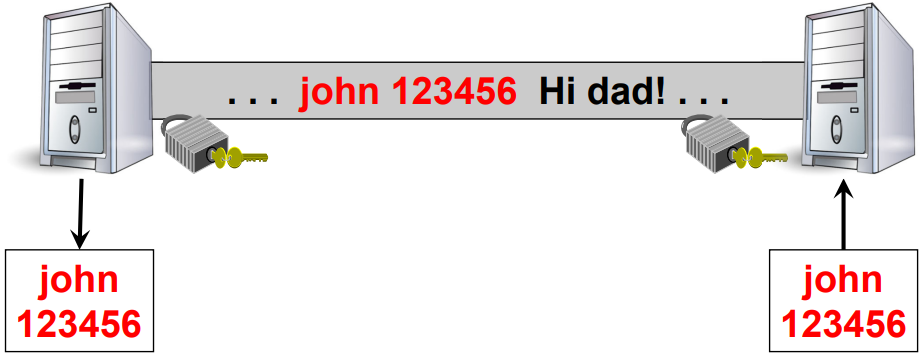
\includegraphics[width=\textwidth]{/home/lorenzo/Notes/Information System Security/images/Screenshot from 2024-12-22 13-22-37.png}
\end{minipage}
\noindent
Since all this features are negotiated \textbf{before transmitting data}, we ensure:
\begin{itemize}
    \item \textbf{Single} or \textbf{mutual authN}
    \item \textbf{Data integrity}
    \item \textbf{Data confidentiality}
\end{itemize}
Channel Security is very easy to implement because it requires no (or small) modification of applications. Since this features are also negotiated \textbf{automatically} we cannot have \textbf{non-repudation}.\\
\\
\textcolor{red}{\textbf{N.B.}} The \textbf{main issue} with Channel Security is that its security properties are provided \textbf{only} during the transit \textbf{inside} the communication channel. So data in \textbf{not} protected when it's located at the end-user. 

\section{Message/Data security}
It applies protection \textbf{only} when it's needed. This means that data is \textbf{individually} protected by wrapping it into a \textbf{secure container}. Data (not the channel) ensures the following security properties:
\begin{itemize}
    \item \textbf{Single authN, not mutual} because features are \textbf{not negotiated}
    \item \textbf{Data integrity}
    \item \textbf{Data confidentiality}
    
\end{itemize}
If protection is applied \textbf{voluntary} and \textbf{explicity} by the user, we can have \textbf{non-repudation}. Message/Data Security requires modification to application.